\documentclass[10pt,landscape,a4paper]{article}
\usepackage[utf8]{inputenc}
\usepackage[ngerman]{babel}
\usepackage[T1]{fontenc}
%\usepackage[LY1,T1]{fontenc}
%\usepackage{frutigernext}
%\usepackage[lf,minionint]{MinionPro}
\usepackage{tikz}
\usetikzlibrary{shapes,positioning,arrows,fit,calc,graphs,graphs.standard}
\usepackage[nosf]{kpfonts}
\usepackage[t1]{sourcesanspro}
\usepackage{multicol}
\usepackage{wrapfig}
\usepackage[top=5mm,bottom=5mm,left=5mm,right=5mm]{geometry}
\usepackage[framemethod=tikz]{mdframed}
\usepackage{microtype}
\usepackage{pdfpages}
\usepackage{amsmath}
\DeclareMathOperator*{\argmax}{\arg\!\max}
\DeclareMathOperator*{\argmin}{\arg\!\min}


\let\bar\overline

\definecolor{myblue}{cmyk}{1,.72,0,.38}

\def\firstcircle{(0,0) circle (1.5cm)}
\def\secondcircle{(0:2cm) circle (1.5cm)}

\colorlet{circle edge}{myblue}
\colorlet{circle area}{myblue!5}

\tikzset{filled/.style={fill=circle area, draw=circle edge, thick},
    outline/.style={draw=circle edge, thick}}
    
\pgfdeclarelayer{background}
\pgfsetlayers{background,main}

\everymath\expandafter{\the\everymath \color{myblue}}
\everydisplay\expandafter{\the\everydisplay \color{myblue}}

\renewcommand{\baselinestretch}{.8}
\pagestyle{empty}

\global\mdfdefinestyle{header}{%
linecolor=gray,linewidth=1pt,%
leftmargin=0mm,rightmargin=0mm,skipbelow=0mm,skipabove=0mm,
}

\newcommand{\header}{
\begin{mdframed}[style=header]
\footnotesize
\sffamily
CZ4041 - Machine Learning
% von~Tim~S.,~Seite~\thepage~von~2
\end{mdframed}
}

\makeatletter % Author: https://tex.stackexchange.com/questions/218587/how-to-set-one-header-for-each-page-using-multicols
\renewcommand{\section}{\@startsection{section}{1}{0mm}%
                                {.2ex}%
                                {.2ex}%x
                                {\color{myblue}\sffamily\small\bfseries}}
\renewcommand{\subsection}{\@startsection{subsection}{1}{0mm}%
                                {.2ex}%
                                {.2ex}%x
                                {\sffamily\bfseries}}



\def\multi@column@out{%
   \ifnum\outputpenalty <-\@M
   \speci@ls \else
   \ifvoid\colbreak@box\else
     \mult@info\@ne{Re-adding forced
               break(s) for splitting}%
     \setbox\@cclv\vbox{%
        \unvbox\colbreak@box
        \penalty-\@Mv\unvbox\@cclv}%
   \fi
   \splittopskip\topskip
   \splitmaxdepth\maxdepth
   \dimen@\@colroom
   \divide\skip\footins\col@number
   \ifvoid\footins \else
      \leave@mult@footins
   \fi
   \let\ifshr@kingsaved\ifshr@king
   \ifvbox \@kludgeins
     \advance \dimen@ -\ht\@kludgeins
     \ifdim \wd\@kludgeins>\z@
        \shr@nkingtrue
     \fi
   \fi
   \process@cols\mult@gfirstbox{%
%%%%% START CHANGE
\ifnum\count@=\numexpr\mult@rightbox+2\relax
          \setbox\count@\vsplit\@cclv to \dimexpr \dimen@-1cm\relax
\setbox\count@\vbox to \dimen@{\vbox to 1cm{\header}\unvbox\count@\vss}%
\else
      \setbox\count@\vsplit\@cclv to \dimen@
\fi
%%%%% END CHANGE
            \set@keptmarks
            \setbox\count@
                 \vbox to\dimen@
                  {\unvbox\count@
                   \remove@discardable@items
                   \ifshr@nking\vfill\fi}%
           }%
   \setbox\mult@rightbox
       \vsplit\@cclv to\dimen@
   \set@keptmarks
   \setbox\mult@rightbox\vbox to\dimen@
          {\unvbox\mult@rightbox
           \remove@discardable@items
           \ifshr@nking\vfill\fi}%
   \let\ifshr@king\ifshr@kingsaved
   \ifvoid\@cclv \else
       \unvbox\@cclv
       \ifnum\outputpenalty=\@M
       \else
          \penalty\outputpenalty
       \fi
       \ifvoid\footins\else
         \PackageWarning{multicol}%
          {I moved some lines to
           the next page.\MessageBreak
           Footnotes on page
           \thepage\space might be wrong}%
       \fi
       \ifnum \c@tracingmulticols>\thr@@
                    \hrule\allowbreak \fi
   \fi
   \ifx\@empty\kept@firstmark
      \let\firstmark\kept@topmark
      \let\botmark\kept@topmark
   \else
      \let\firstmark\kept@firstmark
      \let\botmark\kept@botmark
   \fi
   \let\topmark\kept@topmark
   \mult@info\tw@
        {Use kept top mark:\MessageBreak
          \meaning\kept@topmark
         \MessageBreak
         Use kept first mark:\MessageBreak
          \meaning\kept@firstmark
        \MessageBreak
         Use kept bot mark:\MessageBreak
          \meaning\kept@botmark
        \MessageBreak
         Produce first mark:\MessageBreak
          \meaning\firstmark
        \MessageBreak
        Produce bot mark:\MessageBreak
          \meaning\botmark
         \@gobbletwo}%
   \setbox\@cclv\vbox{\unvbox\partial@page
                      \page@sofar}%
   \@makecol\@outputpage
     \global\let\kept@topmark\botmark
     \global\let\kept@firstmark\@empty
     \global\let\kept@botmark\@empty
     \mult@info\tw@
        {(Re)Init top mark:\MessageBreak
         \meaning\kept@topmark
         \@gobbletwo}%
   \global\@colroom\@colht
   \global \@mparbottom \z@
   \process@deferreds
   \@whilesw\if@fcolmade\fi{\@outputpage
      \global\@colroom\@colht
      \process@deferreds}%
   \mult@info\@ne
     {Colroom:\MessageBreak
      \the\@colht\space
              after float space removed
              = \the\@colroom \@gobble}%
    \set@mult@vsize \global
  \fi}

\makeatother
\setlength{\parindent}{0pt}

\begin{document}
%\footnotesize
\small
\begin{multicols*}{5}

\section{Bayesian Classifiers}
\subsection*{Probabilities}
\subsection*{Sum Rule}
$P(A) = \sum_B P(A,B)$\\
$P(A) = \sum_B\sum_C P(A,B,C)$\\
\subsection*{Product Rule}
$P(A,B) = P(B|A)\times P(A) = P(A|B)\times P(B)$\\
\subsection*{Bayes Theorem}
\[P(A|B) = \frac{P(A,B)}{P(B)} = \frac{P(B|A)P(A))}{P(B)}\]\\
(Generalised case)\\
\[P(A_1...A_k|B_1...B_p) = \frac{P(B_1...B_p,A_1...A_k)}{P(B_1...B_p)}\]\\
\subsection*{Bayesian Classifiers}
Bayesian classifiers aim to find the mapping $f: \mathbf{x} \Rightarrow y$
for supervised learning in the form of conditional probability $P(y|\mathbf{X})$
via Bayes rule.
\[P(y|\mathbf{X}) = \frac{P(y, \mathbf{X})}{P(\mathbf{X})} = \frac{P(\mathbf{X}|y)P(y)}{P(\mathbf{X})}\]\\
For a classification with C classes, given a data instance $\mathbf{x^*}$:\\
\[y^* = c^* if c^* = \argmax_c P(y=c|\mathbf{x^*})\]\\
Applying Bayes rule,\\
\[P(y=c|\mathbf{x^*}) = \frac{P(\mathbf{x^*}| y=c)P(y=c)}{P(\mathbf{x^*})}\]\\
Therefore,\\
\[y^* = \argmax_c \frac{P(\mathbf{x^*}| y=c)P(y=c)}{P(\mathbf{x^*})}\]\\
\[= \argmax_c P(\mathbf{x^*}| y=c)P(y=c)\]\\

\section{Bayesian Decision Theory}
Incorporating cost of misclassification on top of simple Bayesian Classifiers.
\subsection*{Loss/Cost}
Actions: $a_c$, i.e., predict $y=c$\\
Define $\lambda_{ij}$ as the cost of $a_i$ when optimal action is $a_j$. E.g.:\\
$\lambda_{00} = 0$ (predict correctly)\\
$\lambda_{11} = 0$ (predict correctly)\\
$\lambda_{01} = 10$ misclassify 1 as 0\\
$\lambda_{00} = 1$ misclassify 0 as 1\\
\subsection*{Expected Risk}
Expected risk for taking action $a_i$:\\
\[R(a_i|\mathbf{x}) = \sum^{C-1}_{c=0}\lambda_{ic}P(y=c|\mathbf{x})\]\\
To classify, for all actions, calculate expected risk, then choose the action 
with the minimum risk.
\subsection*{Special Case: 0/1 loss}
\[\lambda_{ij} = \begin{cases}
    0 \text{ if } i = j \\
    1 \text{ if } i \neq j
\end{cases}\]
$\therefore R(a_i|\mathbf{x}) = 1 - P(y=i|\mathbf{x})$\\
In this case,\\
\[\text{Choose } a_i \text{ if } R(a_i|\mathbf{x}) = \min_{a_c}R(a_c|\mathbf{x})\]
Is equivalent to:\\
\[\text{Predict } y = c^* \text{ if } P(y=c^*|\mathbf{x}) = \max_{c}P(y=c|\mathbf{x})\]



\section{Na\"{i}ve Bayes Classifiers}
\subsection*{Independence}
A is \textbf{independent} of B, if:\\
$P(A,B) = P(A|B)\times P(B) = P(A)\times P(B)$\\
$P(A,B) = P(B|A)\times P(A) = P(A)\times P(B)$\\
Or,\\
$P(A|B) = P(A)$\\
$P(B|A) = P(B)$\\
\subsection*{Conditional Independence}
A is \textbf{conditionally independent} of B, given C if:\\
$P(A|B,C) = P(A|C)$\\
\subsection*{Na\"{i}ve Bayes Classifier}
1. Assumption: conditional independence of features given label\\
\[p(\mathbf{x}|y = c) = P(x_1,...,x_d|y=c)\]
\[ = P(x_1|y=c)P(x_2|y=c)...P(x_d|y=c)\]
\[ = \prod^{d}_{i=1}P(x_i|y=c)\]
To classify a test record $\mathbf{x^*}$, compute the posteriors for 
each class:\\
\[p(y=c|\mathbf{x^*}) = \frac{(\prod^{d}_{i=1}P(x_i^*|y=c))P(y=c)}{P(\mathbf{x^*})}\]
Since $P(\mathbf{x^*})$ is constant for each class c, it is sufficient 
to choose the class that maximises the numerator term.
\[y^* = \argmax_c (\prod^{d}_{i=1}P(x_i^*|y=c))P(y=c)\]\\

\subsection*{Estimating Cond Prob (Discrete)}
\[P(x_i = k| y = c) = \frac{|(x_i - k)\wedge (y=c)|}{|y=c|}\]
\subsection*{Estimating Cond Prob (Continuous)}
\[P(x_i|y=c) = \frac{1}{\sqrt{2\pi \sigma^2_{ic}}}e^{-\frac{(x_i-\mu_{ic})^2}{2\sigma^2_{ic}}}\]
Supposing there are $N_c$ instances in class c,\\
Sample mean:
\[\mu_{ic} = \frac{1}{N_c}\sum^{N_c}_{j=1}x_{ij}\]
Sample variance:
\[\sigma^2_{ic} = \frac{1}{N_c-1}\sum^{N_c}_{j=1}(x_{ij}-\mu_{ic})^2\]

\subsection*{Laplace Estimate}
Alternative prob estimation for discrete features.
\[P(x_i = k| y = c) = \frac{|(x_i - k)\wedge (y=c)|+1}{|y=c|+n_i}\]
where $n_i$ is \#distinct values of $x_i$.
In extreme cases with no training data, $P(x_i = k| y = c) = \frac{1}{n_i}$\\

\subsection*{M-estimate}
A more general estimation:
\[P(x_i = k| y = c) = \frac{|(x_i - k)\wedge (y=c)|+m\times \tilde{P}(x_i = k| y = c)}{|y=c|+m}\]
Where $m$ is a hyperparameter and $\tilde{P}(x_i = k| y = c)$ is prior information of ${P}(x_i = k| y = c)$. 
(e.g., domain knowledge)

Extreme case with no training data: $P(x_i = k| y = c) = \tilde{P}(x_i = k| y = c)$
\section{Bayesian Belief Networks}
Suppose all features are \textbf{discrete} 
(if there are continuous and discrete, estimation is much more difficult)\\\\
Two key elements:\\
1. A directed acyclic graph (DAG) encoding dependence relationships between 
a set of variables\\\\
2. A probability table associating each node to immediate parent nodes

\subsection*{DAG: Conditional Independence}
A node in a Bayesian network is conditionally independent of its 
non-descendants, \textbf{if its parents are known}.
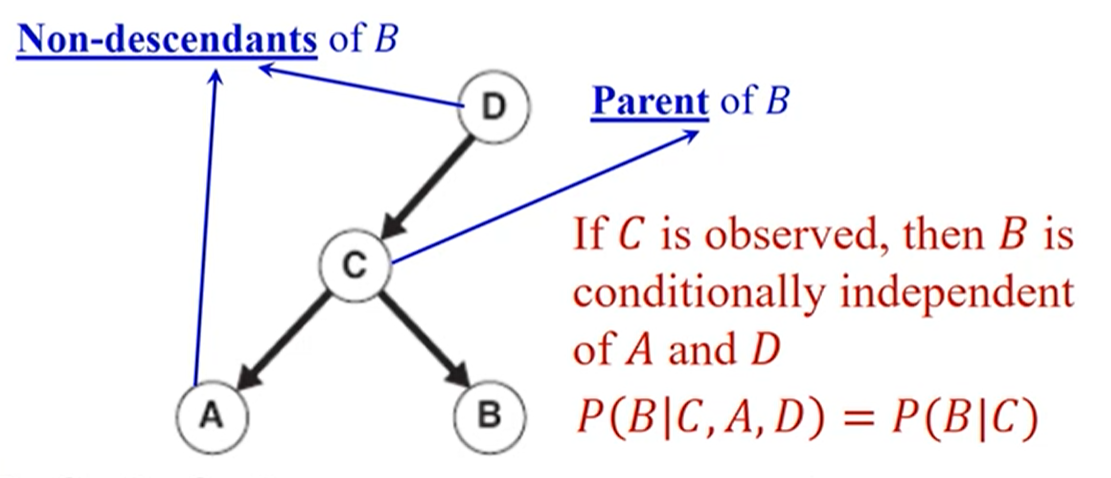
\includegraphics[width=\linewidth]{fig/bbn1}\\\\
\textbf{IMPORTANT!} If A and B are conditionally independent given C, we have:\\
1. $P(A|B,C) = P(A|C)$\\
2. $P(A,B|C) = P(A|C)P(B|C)$
\\

\subsection*{Important! Using BBN for Inference}
Given a BBN, and an inference(prediction) task:\\
1. Translate problem into probabilisitc language\\
2. If the probabilities to be estimated cannot be obtained 
from the probability tables of the BBN, then\\
A. Identify a subgraph which captures the dependence between 
input variables (features) and output variable (class)\\\\
B. Based on the network topology, apply product rule, sum rule
and the properties of conditional independence and independence
to induce equivalent forms of the probabilities until all 
probabilities can be found from the probability tables.

% \input{sections/mengen}
% \input{sections/relationen}
% \input{sections/abbildungen}
% \input{sections/beweise} 
% \input{sections/graphen}
% \input{sections/graphalgo}
% \input{sections/bool}
% \input{sections/formeln}
\end{multicols*}
\end{document}